\subsection{Efecto Ramsauer-Townsend}


Para estudiar el efecto Ramsauer--Townsend se utilizó un módulo equipado 
con un tiratrón 2D21. El filamento del tubo se alimentó mediante una fuente 
de voltaje variable con el propósito de calentar el cátodo y producir emisión 
termoiónica. Por otra parte, se empleó una segunda fuente para controlar el 
voltaje de cátodo \(V_c\). Los voltajes de ánodo \(V_a\) y de 
rejilla-blindaje \(V_{rb}\) se midieron en las terminales correspondientes 
del módulo.\\

La disposición interna del tubo y la polarización de sus electrodos se 
muestran en la Fig.~\ref{fig:conexion-interna}, mientras que las conexiones 
entre el módulo, las fuentes de alimentación y los instrumentos de medición 
se presentan en la Fig.~\ref{fig:montaje-experimental}. Antes de energizar 
el circuito se verificó el funcionamiento de las fuentes y se comprobó que 
sus voltajes de salida se encontraran inicialmente en \(0~\mathrm{V}\).\\

\begin{figure}[h]
    \centering
    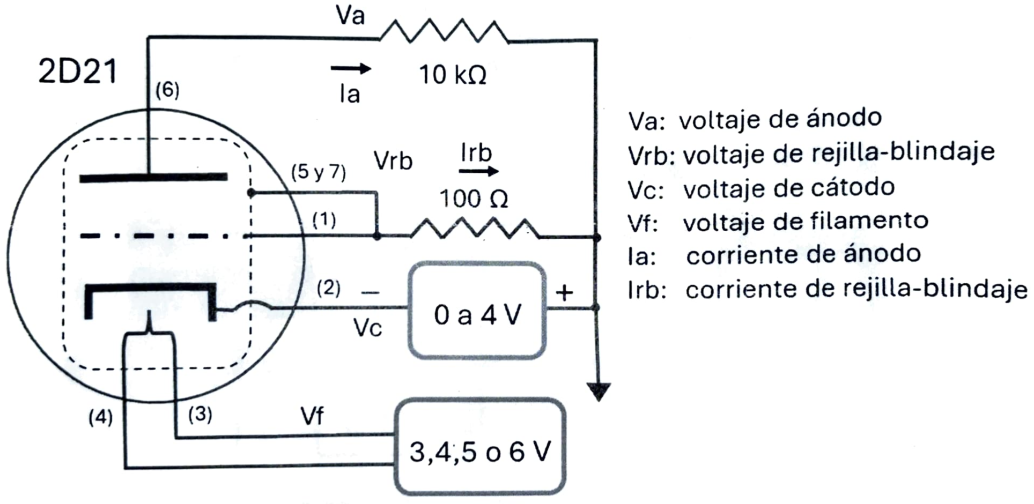
\includegraphics[width=\columnwidth]{figuras/montaje_diag.png}
    \captionof{figure}{Diagrama de conexión interna del módulo con el bulbo 2D21.}
    \label{fig:conexion-interna}
\end{figure}

\begin{figure}
    \centering
    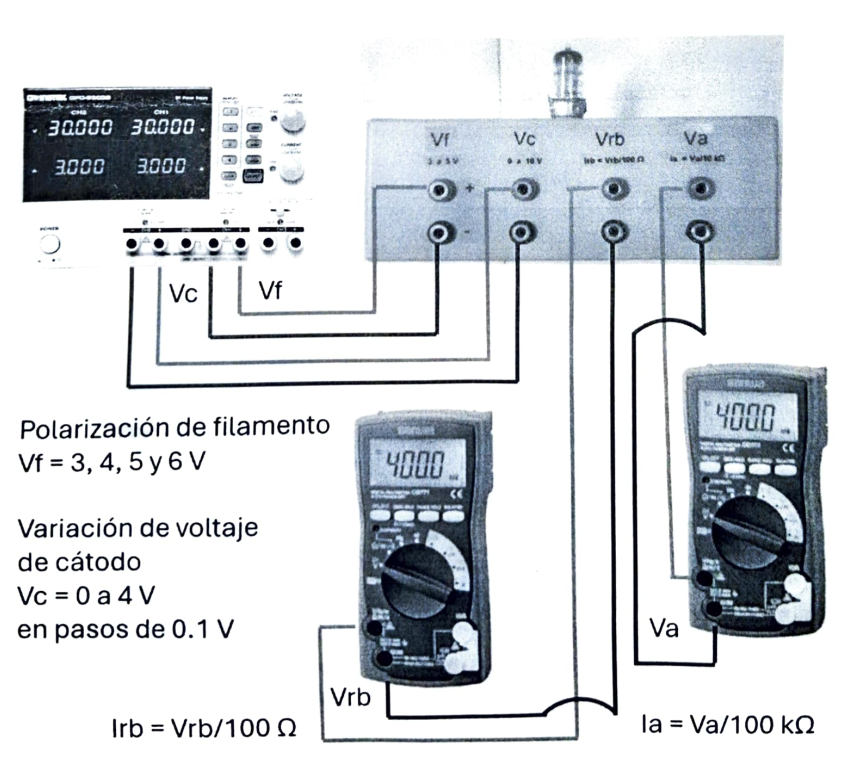
\includegraphics[width=0.95\columnwidth]{figuras/montaje_fisico.png}
    \captionof{figure}{Diagrama de conexión del montaje.}
    \label{fig:montaje-experimental}
\end{figure}

Las mediciones se realizaron para los voltajes de filamento $V_f = 2,\ 3 \text{ y } 4~\mathrm{V}$. Para cada valor de \(V_f\), el voltaje del filamento se incrementó gradualmente desde \(0~\mathrm{V}\) hasta alcanzar el valor bajo estudio. 
Con el voltaje de cátodo inicialmente en \(V_c=0~\mathrm{V}\), se dejó 
calentar el filamento durante aproximadamente cinco minutos para permitir 
la estabilización térmica del cátodo.\\

Posteriormente, se efectuó un barrido del voltaje de cátodo desde 
\(0\) hasta \(4~\mathrm{V}\), con incrementos de \(0.1~\mathrm{V}\), en cada punto del barrido se registraron simultáneamente los voltajes 
\(V_a\) y \(V_{rb}\). Este procedimiento se repitió para cada uno de los 
tres valores de \(V_f\).\\


La adquisición de datos se llevó a cabo mediante dos modalidades. En la 
primera, el barrido de \(V_c\) se realizó manualmente, ajustando la fuente 
en pasos de \(0.1~\mathrm{V}\) y anotando las lecturas de \(V_a\) y 
\(V_{rb}\) indicadas por los voltímetros.\\

En la segunda modalidad se utilizó un programa desarrollado en el 
laboratorio para automatizar el mismo procedimiento. Se introdujo en el 
software el valor deseado de \(V_f\), tras lo cual el sistema realizó el 
barrido de \(V_c\) y generó automáticamente el registro correspondiente de 
\(V_a\) y \(V_{rb}\). En ambas modalidades se conservaron los mismos 
voltajes de filamento, intervalo de barrido e incremento de \(V_c\), con 
el fin de comparar los datos obtenidos manualmente con los adquiridos por el sistema electrónico.


